\chapter{Resultados y validación}

\section{Introducción}
La validación del sistema es una etapa crítica en el proceso de desarrollo de cualquier proyecto, especialmente en un proyecto de la magnitud y complejidad del convertidor diseñado. La validación se encarga de verificar que todos los componentes y subsistemas del convertidor funcionen correctamente y cumplan con los requisitos y especificaciones establecidos previamente.

Dada la naturaleza multifacética del convertidor, que abarca desde aspectos eléctricos y electrónicos hasta aspectos de control y \textit{firmware}, es esencial planificar una estrategia de validación exhaustiva y efectiva. En este sentido, se ha adoptado un enfoque metodológico basado en el modelo en V, que permite validar los subsistemas desde los más específicos hasta los más generales, siguiendo un flujo lógico y sistemático. 

En este capítulo se desarrolla la parte derecha de la 'V', diseñando y ejecutando las pruebas a varios niveles. La estrategia de validación se divide en tres grandes bloques: validación de \textit{hardware}, validación de \textit{firmware} e integración. Cada bloque tiene sus propios desafíos y requisitos específicos, pero todos contribuyen al objetivo final de asegurar el funcionamiento correcto y robusto del convertidor.

\section{Validación de \textit{hardware}}
La parte más crítica en la validación del convertidor es la de \textit{hardware} puesto que cada iteración cuesta tiempo y dinero. Por ello, son las pruebas de \textit{hardware} las que se diseñan y ejecutan más meticulosamente. En particular, se prestó especial atención a la placa de potencia, puesto que es el diseño más complicado de los dos.

Inicialmente, se elaboraron hojas de cálculo detalladas para cada uno de los tests, abarcando desde la inspección visual y pruebas de subcircuitos, hasta la evaluación de sistemas algo más complejos. Sin embargo, a medida que avanzaba el proceso de validación y se integraban los subcircuitos unos con otros, se hizo evidente que un enfoque más dinámico y adaptativo era necesario. Esto se debió a que los problemas encontrados y las soluciones implementadas requerían una validación continua y menos estructurada, lo que permitía realizar ajustes y mejoras en menos tiempo.


\subsection{Pre-inspección de la placa de potencia}
Antes de realizar cualquier prueba funcional, se llevó a cabo una inspección visual exhaustiva de la PCB de potencia para identificar cualquier defecto físico o de manufactura. Esta inspección incluyó la verificación del acabado superficial, la serigrafía, el grosor del cobre en las capas y las dimensiones de la placa. En la primera iteración se encontraron algunos problemas menores, como una serigrafía invertida en los conectores del bus de continua, pero no afectaron las pruebas iniciales.

Se validó el grosor de cobre en las vías para aportar confianza a la hora de montar los componentes \textit{press-fit}. Para ello, se extrajo una sección de la PCB que cortaba transversalmente una vía y se pulió. Posteriormente, se tomó una fotografía con un microscopio y se hicieron medidas digitales.

\begin{figure}[H]
	\centering
	\includegraphics[width=0.7\linewidth]{fig/copperVia1}
	\caption{Extracción de una muestra de la PCB.}
\end{figure}


\begin{figure}[H]
	\centering
	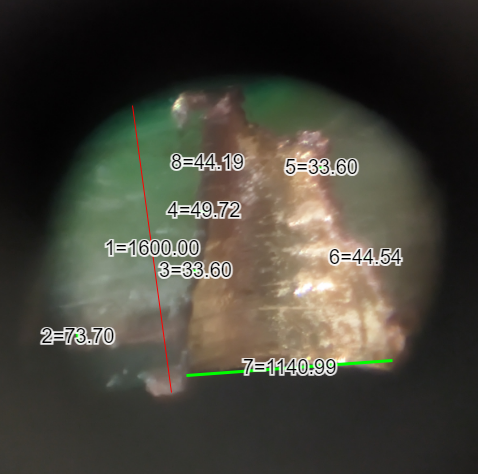
\includegraphics[width=0.7\linewidth]{fig/copperVia}
	\caption{Micrografía de una vía de la placa de potencia. Se pueden apreciar los grosores de cobre en las 4 capas y en la vía.}
\end{figure}

Se pudo comprobar que el grosor de las capas era correcto (70 micras), y que el de las vías estaba dentro de la tolerancia establecida (de 25 a 50 micras).

\subsection{Primer contacto con la placa de potencia}

Durante la primera interacción con la placa de potencia, se realizaron diversas pruebas para validar el funcionamiento de los distintos componentes y subcircuitos de forma aislada. Principalmente se busca validar una funcionalidad básica de cada uno de forma separada, de manera que si se encuentran problemas de integración se sepa que son de integración y no de los componentes o circuitos individuales. Se ordenaron estas pruebas de "dentro hacia afuera", empezando por el circuito de \textit{driving} y acabando con la interacción externa del mismo. También se validó la adquisición de variables analógicas y se probó la funcionalidad básica del circuito de descarga.


\subsubsection{Alimentación del \textit{gate driver}}

Para validar la alimentación del \textit{gate driver} se separó en una verificación del LDO para la tensión negativa por separado, y en otra para validar el DC-DC.

En primer lugar se pobló únicamente el propio LDO con los componentes necesarios para su funcionamiento. Se anotó el primer error de la placa, que consiste en una equivocación en el mapeado de los pines del esquemático al \textit{footprint}. De todas formas, se realizó un \textit{dead-bugging} para conectar el componente de forma correcta y poder verificar el circuito de forma exitosa.

\begin{figure}[H]
	\centering
	\includegraphics[width=0.7\linewidth]{fig/deadbug}
	\caption{LDO \textit{dead-bugged} con resina para evitar daños con las siguientes pruebas.}
\end{figure}

\begin{itemize}
	\item \textbf{Valor esperado}: -4 V $\le$ V $\le$ -3.5 V
	\item \textbf{Resultado}: -3.78 V
\end{itemize}


La dificultad de realizar este \textit{rework} fue motivo suficiente para corregir el diseño, pero se esperó a finalizar la mayoría de pruebas básicas antes de pedir placas nuevas.

Después de verificar el funcionamiento del LDO se probaron los DC-DCs aislados. Funcionaron según lo previsto, aunque se notó que se calentaban ligeramente, incluso en vacío (sin carga). Esto se debe a su curva de rendimiento, que con cargas bajas es muy poca. Además se anotaron variaciones en las tensiones de salida, pero resultó que eran función de la carga, y está explicado en la hoja de datos.

\begin{figure}[H]
	\centering
	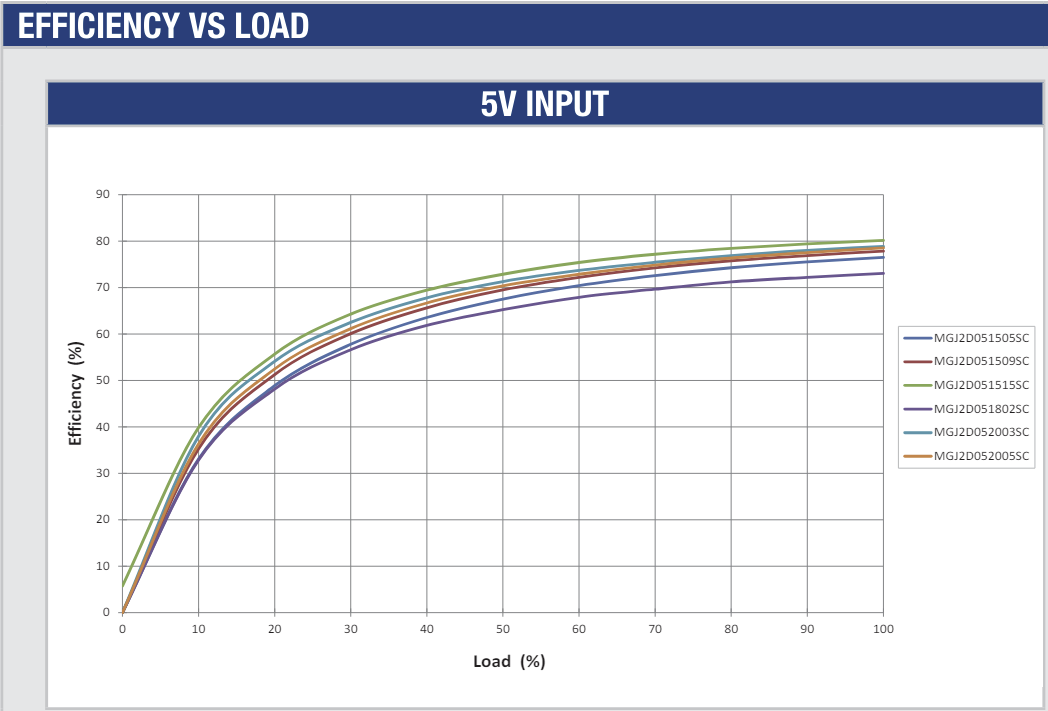
\includegraphics[width=0.7\linewidth]{fig/DCDC-eff}
	\caption{Curva de rendimiento del DC-DC aislado.}
\end{figure}

\begin{figure}[H]
	\centering
	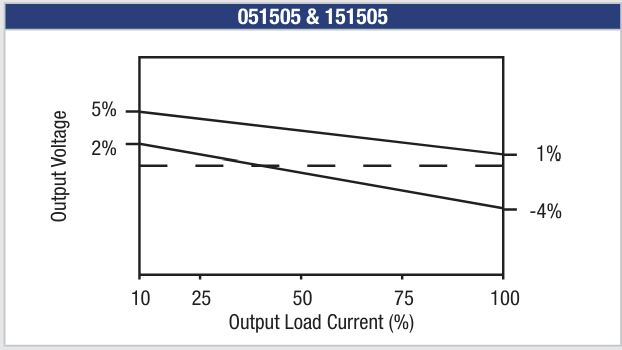
\includegraphics[width=0.7\linewidth]{fig/DCDC-eff1}
	\caption{Variación de la tensión de salida en función de la carga.}
\end{figure}

\begin{itemize}
	\item \textbf{Valor esperado}: 15.5 V $\le$ VDD $\le$ 14.5 V ; -4 V $\le$ VEE $\le$ -3.5 V
	\item \textbf{Resultado}: 15.94 V ; -3.78 V
\end{itemize}

\subsubsection{Funcionalidad del \textit{gate driver}}
Para validar la funcionalidad básica del \textit{gate driver}, se montó un módulo de potencia y los dos \textit{gate drivers} necesarios para controlar los dos MOSFETs.

\begin{itemize}
	\item \textbf{\textit{OK} y \textit{TRIP}}: Se poblaron los componentes necesarios y se alimentó la placa desde el lado de LV. Se midieron los nodos TRIP y OK. Ambas señales tenían un valor de 5V, confirmando su correcto funcionamiento sin errores. Posteriormente se forzaron fallas en el lado del semiconductor y ambas bajaron a 0V.
	\item \textbf{Dispositivos apagados en reposo}: Se montaron las resistencias de puerta y se verificó el estado de ambos MOSFETs midiendo la resistencia entre \textit{drain} y \textit{source}. Ambos dispositivos se encontraban en estado \textit{OFF}, confirmando que no se encendían.
	\item \textbf{\textit{Enable} no enciende los dispositivos}: Se introdujo una señal de 3.3V el nodo ENABLE. De nuevo, ambos dispositivos se encontraban en estado \textit{OFF}, lo cual es el resultado esperado, ya que ambas señales de PWM estaba en estado bajo, es decir, consignando que los MOSFETs estuvieran abiertos.
	\item \textbf{Medición de temperatura}: Se verificó la capacidad del \textit{gate driver} de tomar una medida analógica, en concreto, de la NTC interna del semiconductor. Se contrastaron las medidas obtenidas con los cálculos previos, arrojando resultados satisfactorios.
	
	\begin{figure}[H]
		\centering
		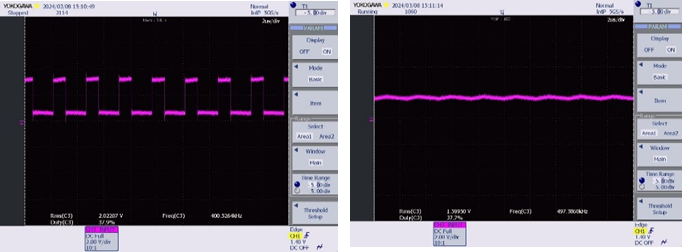
\includegraphics[width=0.7\linewidth]{fig/NTC-driver}
		\caption{Medición de temperatura ambiente. Se puede ver la señal de salida sin filtrar (PWM) y filtrada.}
	\end{figure}
	
\end{itemize}
	
\subsubsection{Sensado de corriente}

Para validar el funcionamiento del sensado de corriente, se realizaron las siguientes pruebas:

\begin{itemize}
	\item \textbf{Standby}: Se esperaba una salida de 2.5V con un margen de error de $\pm$ 5 mV. La salida medida fue de 2.499 V, lo que se considera dentro del rango aceptable.
	
	\item \textbf{Operación básica}: Se esperaba una salida de 2.5625V para una corriente de +5A y 2.4375V para una corriente de -5 A, con un margen de error de $\pm$ 5 mV. Las mediciones obtenidas fueron de 2.557 V para +5 A y 2.436 V para -5 A, ambas dentro del rango esperado.
\end{itemize}	


\subsubsection{Descarga}

Para verificar la funcionalidad de la descarga, se realizaron las siguientes pruebas:

\begin{itemize}
	\item \textbf{Descarga pasiva}: Se precalculó una descarga de 24 V a 10 V en 35 segundos usando un 20\% de la capacidad del bus. La medición obtenida fue de 5.5 segundos, debido a que no se tuvo en cuenta el resto de conexiones entre los terminales positivo y negativo. La resistencia aparente entre estos terminales era más baja, principalmente por el divisor de tensión usado para tomar la medida de voltaje del bus. El divisor de voltaje para la adquisición ya es de $6 \cdot 68 \text{ k}\Omega + 4.7 \text{ k}\Omega = 412.7 \text{ k}\Omega$, y está en paralelo con la resistencia de $2 \text{ M}\Omega$, lo que resulta en una resistencia equivalente de 
	$$
	\frac{1}{\frac{1}{2 \text{ M}\Omega} + \frac{1}{412.7 \text{ k}\Omega}} = 342 \text{ k}\Omega,
	$$
	lo que equivale a aproximadamente 6 segundos de descarga. Al agregar cualquier otra resistencia en paralelo, como la de los propios semiconductores u otros componentes, los cálculos coinciden.
	
	\begin{figure}[H]
		\centering
		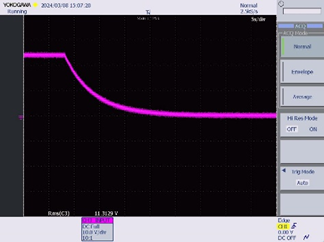
\includegraphics[width=0.7\linewidth]{fig/discharge1}
		\caption{Descarga pasiva a 24 V con 20 $\mu$F.}
	\end{figure}
	
	\item \textbf{Control de la descarga}: Se aplicó un voltaje de 20V en el nodo \textit{SC\_END} y se suministraron 24 V entre \textit{TS+} y \textit{TS-}. Se esperaba que la diferencia de potencial entre \textit{TS+} y \textit{TS-} fuera de 10 V 0.35 segundos después de retirar el voltaje, que coincidió perfectamente con el cálculo previo.
	\begin{figure}[H]
		\centering
		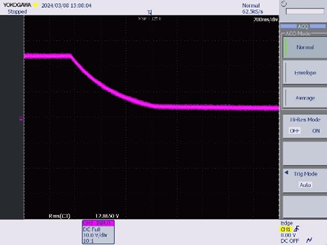
\includegraphics[width=0.7\linewidth]{fig/discharge2}
		\caption{Descarga activa a 24 V con 20 $\mu$F. Se puede ver como a 10 V (la tensión del zener) se desactiva la descarga activa.}
	\end{figure}
\end{itemize}
	
	
\subsubsection{Sensado de voltaje}

Para verificar el sensado de voltaje, se llevaron a cabo las siguientes pruebas:

\begin{itemize}
	\item \textbf{Divisor de voltaje}: Se aplicaron 24 V entre \textit{TS+} y \textit{TS-}. Se capturó el voltaje en el divisor de tensión. La tensión esperada era de $0.011388 \cdot 24\text{ V} = 0.2733 \text{ V}$ con un margen de error de $\pm$1 mV. La medición obtenida fue de 0.272 V, dentro del rango aceptable.
	
	\item \textbf{Alimentación aislada}: Se montó el convertidor DCDC501 y se alimentó la placa desde el lado LV para medir el voltaje entre \textit{+5\_TS} y \textit{TS-}. Se esperaba una lectura de 5V con un margen de error de $\pm$0.5 V. Sin embargo, la medición fue de 5.5 V, indicando que se deberá ajustar el divisor de voltaje para el umbral de detección debido a la inexactitud.
	
	\item \textbf{Detección de voltaje}: Se aplicaron 50 V entre \textit{TS+} y \textit{TS-}, y se midió \textit{TSAL\_ON}. Se repitió la prueba con 60 V. Se esperaba que \textit{V\_TSAL} fuera de 677 mV y que \textit{TSAL\_ON} fuera 5 V con 50 V de tensión de bus y 0 V con 60 V. Sin embargo, la medición fue incorrecta, ya que el umbral aproximado para la transición fue de 63 V. Se encontró que la causa podría estar la tolerancia del divisor de resistencia y el hecho de que la salida del convertidor DC-DC era medio voltio superior.

	\item \textbf{Sensado de voltaje}: Se aplicaron 13V entre \textit{TS+} y \textit{TS-}. Se capturó el valor entre \textit{VDC\_sns+} y \textit{VDC\_sns-}. Se esperaba que la diferencia de potencial fuera de 0.0495 V. La medición obtenida fue de 0.05 V, dentro del rango aceptable.
\end{itemize}


\subsubsection{Resumen de errores encontrados y revisión de la PCB}

Se encontraron los siguientes errores durante el proceso de prueba y montaje:

\begin{enumerate}
	\item \textbf{Problema:} El serigrafiado de los conectores de alimentación (+ y -) está invertido. Esto no afecta las pruebas. \\
	\textbf{Solución propuesta:} Nombrar los conectores según corresponda y cambiar los textos del serigrafiado. Pedir nuevas PCBs.
	
	\item \textbf{Problema:} Se conectó accidentalmente el nodo de 5 V de alimentación a \textit{SC\_END} (20 V), lo  que hizo que todos los componentes alimentados a 5 V murieran.\\
	\textbf{Solución propuesta:} Añadir protecciones a la alimentación de 5 V.
	
	\item\textbf{Problema:} El \textit{footprint} del LDO tiene los pines 4 y 5 intercambiados (\textit{-VEE}, \textit{FB}). \\
	\textbf{Solución propuesta:} Montar el LDO verticalmente con conexiones flotantes cruzadas.
\end{enumerate}

Para realizar el resto de pruebas se pidieron nuevas placas, con las siguientes modificaciones:

\begin{itemize}
	\item Protecciones para la alimentación de 5 V.
	\item Se intercambiaron los pines 4 y 5 en los LDO de los \textit{gate drivers}.
	\item Se intercambiaron \textit{MP+} y \textit{MP-} junto con su serigrafiado.
	\item Se añadieron \textit{testpoints} para la referencia de los sensores de corriente.
	\item Se añadieron \textit{testpoints} para \textit{VDC\_sns+} y \textit{VDC\_sns-}.
	\item Se renombraron los \textit{testpoints} en el esquemático de los \textit{gate drivers} para agilizar las pruebas.
	\item Se añadieron varios textos e indicaciones en el serigrafiado.
\end{itemize}

\subsection{Conmutación de una rama como DC-DC síncrono}
	
\subsection{Pruebas térmicas y de alta tensión}

\subsection{Validación de la placa de control}


\section{Validación de \textit{firmware}}
\subsection{Verificación de los periféricos}

\subsection{Conmutación de las tres ramas}

\subsection{Lazo abierto de tensión con carga R-L}

\subsection{Lazo abierto de tensión con un motor}

\subsection{Lazo cerrado de corriente con carga R-L}

\subsection{Adquisición de la posición del motor}

\subsection{Lazo cerrado de corriente con un motor}

\subsection{Trayectorias de control}

\subsection{Control dual}

\section{Integración}
